%
% File: chap02.tex
% Author: Oliver J. H. Feighan
% Description: delta-scf benchmarking, including dft and dftb methods.
% Talk about important factors for modelling LHII
%
%\let\textcircled=\pgftextcircled
\chapter{Mean-Field excited states}
\label{chap:dscf}

\subsubsection*{Previous Published Work}
Some of the work presented in this chapter forms part of a paper published with 
Dr Susannah Bourne-Worster, in March 2021\cite{Worster2021}. The account given in this 
chapter includes research that was also reported in this publication, namely the
parts of section \ref{sec:benchmarking} from \ref{subsec:reference_data} up to
but excluding \ref{subsec:dscf_gfn_tests}.

\initial {T}his chapter investigates the accuracy of \dscf methods with  both an 
ab initio DFT level of theory as well as with semi-empirical, tight-binding
approximations. The reduced cost and moderate accuracy of these methods
make them an ideal substitute for full TD-DFT or high-level methods when investigating
large systems like chlorophyll.
Transition properties were calculated for a range of molecules, as well as
for a small set of chlorophyll geometries, using variety of different basis sets,
density functionals, response methods and electronic structure methods. Most of 
the work was compared to either high-standard EOM-CCSD or SCS-CC2 reference, from
which conclusions were made on the accuracy of each method. The non-orthogonality 
issue of the ground and excited states was also investigated for the mean-field 
\dscf method. 
Aassigning the symmetries of transitions was also investigated to improve the workflow
of comparing \dscf and TD-DFT results.
It was found that while the DFT methods give reasonable results, the semi-empirical
\dscf methods are not as accurate.

\dscf is a well-known method for calculating transition energies, as well as
ionisation potentials, electron affinities and other properties. Although slightly
less accurate than other high-level response theories, it is much more efficient,
requiring only two SCF solutions for the two states of a transition. In the context 
of calculating large volumes of transition properties for the chlorophyll sites of
LHII, this efficiency makes it a good candidate for investigation.

Previous work in the literature has discussed the benefits of the \dscf method for 
large scale systems. Notably 

%=======
\section{Theory}
\label{sec:dscf_theory}
\subsection{$\Delta$-SCF}
\label{subsec{dscf_and_eigdiff}}

\dscf predicts the transition energy $\Delta E$ of a system as the difference of
the single point energy $E_n$ of two states:

\begin{equation}
\Delta E = E_{2} - E_{1}
\end{equation}
%
It is usually assumed that the excited state solution will be in a similar
location to the ground state in the MO coefficient space. The ground state MO 
coefficients are usually used for an initial guess for the excited
state for this reason. In its simplest form, the \dscf method calculates
the ground state with normal DFT or other mean-field methods, and
then calculates the excited state by rerunning the same method with the excited
state occupation numbers. The two sets of MO coefficients give a full description
of both the ground as excited state.

The issue with finding the excited state solution is that the variation principle
and SCF iterative procedure will try to find the global minimum, which is the 
ground state. The excited state is a local minimum, and so often is less reliable
to find as a solution, especially from the standard SAD initial guess.
For this reason it is often found that converging to the \dscf excited state will
fail. Even when using the ground state as an initial guess with excited state
occupations, normal SCF procedure may still collapse back to the ground state.
Usually it is necessary to include additional changes to the SCF procedure,
such as Fock damping, alternative DIIS methods and sometimes intermediate 
initial guess steps.

Initially, the excited state was calculated by relaxing the orbitals which
contain the excited electron and hole in the ground state space, so that the
excited state and ground state are orthogonal \cite{Hunt1969}. However, it was
argued that this procedure would exacerbate the likelihood of collapsing to the ground
state, and that the excited state was not a proper SCF solution \cite{Gilbert2008}.
Alternatively, an SCF like method was proposed, where instead of
populating orbitals according to the Aufbau principle, orbitals which most
resemble the previous iteration's orbitals should be occupied. This is known as 
the maximum overlap method (MOM). In the maximum overlap method, each iteration 
in an SCF procedure produces new molecular orbital coefficients by solving the 
Roothaan-Hall equations \cite{Roothaan1951}, generally given as an eigenvalue problem:

\begin{equation}
\mathbf{F} \mathbf{C}^{\text{n}} = \mathbf{S} \mathbf{C}^{\text{n}} \epsilon
\label{eq:roothaan_hall}
\end{equation}
%
where $\mathbf{C}^{\text{n}}$ are the $n^{\text{th}}$ orbital coefficient solutions, 
$\mathbf{S}$ is the overlap of orbtials, and $\epsilon$ are the orbital energies. 
The Fock matrix $\mathbf{F}$ is calculated from the previous set of orbital 
coefficients,

\begin{equation}
\mathbf{F} = f\left(\mathbf{C}^{n-1}\right)
\end{equation}
%
. The amount of similarity of orbitals can be estimated from their overlap,

\begin{equation}
\mathbf{O} = \left(\mathbf{C}^{\text{old}}\right)^\dagger \mathbf{S} \mathbf{C}^{\text{new}}
\end{equation}
%
and for a single orbital can be evaluated as a projection,

\begin{equation}
p_j = \sum^n_i O_{ij} = \sum^N_\nu \left[\sum^N_\mu\left(\sum^n_i C_{i\mu}^{\text{old}}\right)S_{\mu\nu}\right]C^{\text{new}}_{\nu j}
\end{equation}
%
where $\mu,\nu$ are orbital indices. the set of orbitals with the highest projection
$p_j$ are then populated with electrons.  This method can be used for any
excited state, with the caveat that the orbital solution will most likely be in
the same region as the ground state solution. For a small number of low lying states,
this is generally  true, and so \dscf can be used to calculate a small spectrum of
excited states \cite{Gilbert2008}.

\dscf has been shown to be cheap alternative to TD-DFT and other higher level
methods \cite{Liu2004, Gavnholt2008, Besley2009}, without considerable losses of
accuracy in certain cases, especially for HOMO-LUMO transitions \cite{Kowalczyk2011}.
Additionally, as the excited state is given as solutions to SCF equations,
the gradient of this solution can be given by normal mean-field theory.
These gradients would be much cheaper than TD-DFT or coupled cluster methods, 
which is advantageous for simulatings dynamics \cite{Gavnholt2008}.

\subsection{Eigenvalue Difference}
\label{subsec:eigval_diff}
Another approximation to full response theory is the eigenvalue difference method. 
Here there is assumed to be no response of the orbital energies and shapes when 
interacting with light. This would be recovered from the complete Cassida equation
if the coupling elements in the $\mathbf{A}$ and $\mathbf{B}$ matrices were set to zero.
Within this approximation, the transition energy is just the difference between 
the ground state energy of the orbital an electron has been excited to($\epsilon_{\text{e}}$)
and the orbital has been excited from ($\epsilon_{\text{g}}$),

\begin{equation}
\Delta E = \epsilon_{\text{e}} - \epsilon_{\text{g}}
\end{equation}
%
. Additionally, transition properties can be calculated by constructing transition 
density matrices from the ground state orbitals such that needing only a single 
SCF optimization is required. Generally, eigenvalue difference methods are not 
seen as accurate response methods, but can offer a quick and easy initial value 
\cite{Gimon2009}.

\subsection{Transition Density and Dipole Moments}
\label{subsec:dscf_transition_density}
\dscf transition properties, such as the transition dipole moment, can be calculated from
the SCF solutions for the ground and excited states. The reduced one-particle transition
density matrix $\mathbf{D}^{21}$ can be written as

\begin{equation}
\mathbf{D}^{21} = \ket{\Psi_1} \bra{\Psi_2}
\end{equation}
%
where $\ket{\Psi_n}$ is the Slater determinant of state $n$, constructed from the
set of spin orbitals $\{ \phi_{j}^{\left(n\right)} \} $. Expressed 
in terms of the molecular orbitals coefficients $\mathbf{C}^{\left(n\right)}$, the
transition density matrix is

\begin{equation}
\mathbf{D}^{21} = \mathbf{C}^{\left(2\right)} \text{adj}\left(\mathbf{S}^{21}\right) \mathbf{C}^{\left(1\right) \dagger}
\end{equation}
%
where $\mathbf{S}^{21}$ is an overlap matrix with elements 

\begin{equation}
S^{21}_{jk} = \braket{\phi^2_j|\phi^1_k}
\end{equation}
%
. The depednece on the adjunct of the overlap
can be understood using L{\"o}wdin's normal rules for non-orthogonal determinants \cite{Lowdin1955}.
In the same way, the transition dipole moment is given by

\begin{equation}
\braket{\Psi_2|\hat{\mathbf{\mu}}|\Psi_1} = \sum_{jk} \mathbf{\mu}_{jk}^{21} \text{adj} \left( \mathbf{S}^{21}\right)_{jk}
\end{equation}
%
where $\hat{\mathbf{\mu}}$ is the one-electron transition dipole operator, and
$\mu_{jk}$ is the element of this operator corresponding to orbital indices $j$, $k$.
The determinant of $\mathbf{S^{21}}$ can be defined as the inner product of the 
two states involved in the transition

\begin{equation}
\left\lvert {\mathbf{S}^{21}} \right\rvert = \braket{\Psi_2|\Psi_1}
\end{equation}

The general definition of the transition dipole

\begin{equation}
\mathbf{\mu}^{1\rightarrow2} = \braket{\Psi_2|\hat{\mathbf{\mu}}|\Psi_1}
\end{equation}

can be expressed with this transition density matrix as:

\begin{equation}
\begin{split}    
\braket{\Psi_2|\hat{\mathbf{\mu}}|\Psi_1} &= \text{tr}\left(\hat{\mathbf{\mu}} \ket{\Psi_1} \bra{\Psi_2} \right) \\
&= \text{tr}\left( \hat{\mathbf{\mu}} \mathbf{D}^{21}\right)
\end{split}
\end{equation}

\subsection{Semi-empirical extensions}
\label{subsec:dscf_xtb}
A main investigation of this chapter is whether the range of DFT methods
that could be used for \dscf and eigenvalue difference methods could be extended 
by using tight-binding methods to predict transition properties.
This mainly focused on the recently published GFN-xTB method, parameterized by
the Grimme group \cite{Grimme2017}. This method has been parameterized for geometries,
frequencies and non-covalent interactions, and uses an extended version of H{\"u}ckel theory.
The name GFN-xTB is an acronym for "Geometries, Frequencies, Non-Covalent - eXtended Tight Binding".
This method was chosen as a similar method has already been published that calculates
transition properties, the precursor to the GFN-xTB methods. This is the sTDA-xTB
method.
Additionally it was convenient the GFN-xTB method was already implemented in the
\code{QCORE} package. This significantly reduced the amount of effort required
for this project, with other users and developers who could help with implementation
of this new method.

\subsubsection{sTDA-xTB}
\label{subsubsec:stda_xtb}
sTDA-xTB ("simplified Tann-Dancoff Approximation - eXtended Tight Binding") is another
method in the family of xTB methods developed by the Grimme group, and is parameterised
for transition properties \cite{Grimme2016}. The accuracy in calculating transition energies with this
method is very good, with the error compared to high-level method, such as SCS-CC2,
being around 0.3 - 0.5 eV.

Similar to other xTB methods, the sTDA-xTB method is a tight-binding method that
uses empirically fitted parameters and a minimal basis set. It was trained on a
test set of highly accurate coupled cluster and density functional theory
excitation energies, as well as atomic partial charges for inter-electronic interactions.

Unlike other xTB methods, coefficients in the basis set for sTDA-xTB are dependent on the D3
coordination number. This makes basis functions far more flexible, which would usually
be achieved with fixed basis functions by using diffuse or other additional orbitals in
the basis set. Additionally, it uses two sets of parameterized basis sets - a
smaller valence basis set (VBS) and an extended basis set (XBS). Whilst this reduces
the cost of having larger basis sets, it makes calculating the gradient of transition
properties much more difficult. This motivates the work on designing an alternative
method with more tractable gradients, instead of using this already established method.

The two basis sets are used to construct formally similar Fock matrix elements,
although in practice they use different global parameters. The core Hamiltonian
is similar to other DFTB methods that use a self-consistent charge (SCC) method, as
opposed to an SCF method, to obtain molecular orbital coefficients. It is given by,

\begin{equation}
\bra{\psi_\mu} H^{\text{EHT, sTDA-xTB}} \ket{\psi_\mu}= \frac{1}{2} \left(k^l_\mu k^{l'}_\nu\right) \frac{1}{2} \left(h^l_\mu h^{l'}_\nu\right) S_{\mu\nu} - k_T \bra{\psi_\mu}\hat{T}\ket{\psi_\nu}
\end{equation}
%
where $\mu,\nu,l,l'$ are orbital and shell indices, $k^l_\mu$ are shell-wise 
H{\"u}ckel parameters, $h$ are effective atomic-orbital energy levels, $S_{\mu\nu}$
is the overlap of orbitals $\mu$ and $\nu$, $k_T$ is a global constant and $\hat{T}$
is the kinetic energy operator. The charges used in the inter-electronic repulsion 
function are given by charge model 5 (CM5) \cite{Marenich2012} charges for the XBS
Fock matrix. These are calculated using Mulliken charges obtained from diagonalising
the Fock matrix with the VBS. The charges for the initial VBS Fock matrix are based
on Gasteiger charges \cite{Gasteiger1978}, modified by the parameterised
electronegativities of atoms in the system.

The whole process for determining molecular orbitals can be summarized as:
\begin{enumerate}
	\item Calculate modified Gasteiger charges for the first initial guess
	\item Diagonalise Fock matrix in the VBS to get the first set of Mulliken charges
	\item Compute CM5 charges
	\item Diagonalise Fock matrix in the VBS again for final set of Mulliken charges.
	\item Recalculate CM5 charges with this final set, and diagonalize the Fock matrix in the XBS. The molecular orbital coefficients from this are then fed to the response theory.
\end{enumerate}

The response theory for this method is based on previous work in the Grimme 
group on the simplified Tamm-Dancoff Approximation \cite{Grimme2013}.
There are several approximations made between full linear response theory and
the sTDA method. First is the Tamm-Danncoff approximation, where the $\mathbf{B}$
matrix is ignored. The second approximation is to use monopole approximations with
Mataga-Nishimoto-Ohno-Klopman (MNOK) operators instead of explicit 2 electron integral
as well as neglecting the density functional term.

Transition charges are used to calculate these MNOK integrals. The charge $q^A_{nm}$
centred on atom $A$ associated withthe transition from $ n \rightarrow m$, are
computed using a Löwdin population analysis:

\begin{equation}
q_{nm}^A = \sum_{\mu \in A} C^\prime_{\mu n} C^\prime_{\mu m}
\end{equation}

where the transformed coefficients $C^\prime_{\mu n}$ are given by orthogonalising
the original MO coefficients $\textbf{C}$:

\begin{equation}
\textbf{C}^\prime = \textbf{S}^{\frac{1}{2}} \textbf{C}
\end{equation}

and $\mu$ is an index that runs over the atomic orbitals (AO). The MO coefficients
are the solution of diagonalising the Fock matrix, similar to equation \ref{eq:roothaan_hall}.

Approximations to full 2 electron integrals are given by charge-charge interaction
damped by the MNOK\cite{Nishimoto1957}\cite{Ohno1964}\cite{Klopman1964} functions.
For exchange and coloumb type integrals, difference exponents are used, along with
an additional free parameter to recover the amount of Fock exchange mixing in
the original matrix element equation. These will be discussed in more detail in
the next chapter, as they are a crucial part of designing a new response method 
for chlorophyll systems.

Third is the truncation of single particle excited space that is used to construct 
the $\mathbf{A}$ matrix. This reduces the number of elements that need to be 
calculated, and so reduces the time taken for diagonalisation, whilst also capturing 
a broad enough spectrum of excitation energies. The sTDA-xTB has many of the same 
goals as this project, except in one respect, which is the gradient theory. As 
the sTDA-xTB method still requires constructing and diagonalizing the $\mathbf{A}$ 
matrix, albeit with a tight-binding method for molecular orbital coefficients, 
the gradient of the transition properties would still be difficult to calculate.

\section{Benchmarking}
\label{sec:benchmarking}
Full scale chlorophyll molecules are too large to be able to calculate a high-level
benchmark. A test set of small molecules, which would cover the same range of elements
as found in organic chromophores and biological molecules, was then chosen as 
it would be able to benchmark both the \dscf methods as well as TD-DFT. With an 
accurate idea of how reliable TD-DFT is, it would be possible to then compare 
\dscf to TD-DFT for chlorophyll systems, as both methods have usable scaling to
calculate transition properties for larger systems, 

The test set chosen was previously used by the Grimme group to parameterise and
test the sTDA-xTB method \cite{Grimme2017}, and was constructed with the same goals
as this work.

\subsection{Reference Data and test set}
\label{subsec:reference_data}
The test set consisted of 109 small molecules. Each system was closed-shell, 
contained 12 atoms or less, and contained on H, C, N, O and F atoms. The size and
specificity of this test set was chosen to minimise any other factors that
could cause errors in analysing the results, whilst still covering all relevant elements
and chemical environments for organic and biological chromophores.

Reference data was calculated as the three lowest energy singlet excited states, 
using EOM-CCSD with an aug-cc-pVTZ basis set. These results were generated
using the Gaussian 16 program \cite{Gaussian16}.

\subsection{Small Systems}
\label{subsec:smalltest}
Transition properties for this test set were calculated using TD-DFT and \dscf,
both using a CAM-B3LYP functional and aug-cc-pVTZ basis set. The transitions were
assigned to the EOM-CCSD results by comparing transition dipoles, energies and 
the character of the MOs involved in the transitions. Where the symmetries could
be assigned, these were also used, but this was not the case for all systems
as many were unsuccessful in labelling symmetry or defaulted to a non-Abelain group.
Symmetry labelling was also only available for TD-DFT calculations, as these were
performed with Gaussian 16. \dscf calculations were done with the \code{QCORE}
program.

The \dscf singlet transition is not a correct representation of a 
true singlet excitation, which is a superposition of both spin-conserving
 $\alpha \rightarrow a, \alpha$ and spin-flipping $\alpha \rightarrow a, \beta$
excitations. The spin-purification formula:

\begin{equation}
\Delta E_S = 2\Delta E^{i,\alpha \rightarrow a, \alpha} - \Delta E^{i,\alpha \rightarrow a, \beta}
\end{equation}

was used to correct for the true singlet excitation energy $\Delta E_S$ \cite{Ziegler1977}.

The results of comparing transition energies and transition dipole magnitudes are
shown in figures \ref{fig:energy_scatter} and \ref{fig:dipole_scatter}.

\begin{figure}
\centering
\includegraphics[scale=0.6]{../../Year_3/dscf_figures/energy_scatter.png}
\caption{Transition energies $\Delta E$ from TD-DFT (black) and \dscf (red)
 plotted against EOM-CCSD energies, with the line $y=x$ (dashed) for reference.
 The ethene dimer outlier has been circled.}
\label{fig:energy_scatter}
\end{figure}

\begin{figure}
\centering
\includegraphics[scale=0.6]{../../Year_3/dscf_figures/dipole_scatter.png}
\caption{Transition dipole magnitudes from TD-DFT (black) and \dscf (red) plotted
against EOM-CCSD transition dipole magnitudes, with the line $y=x$ (dashed) for 
reference.}
\label{fig:dipole_scatter}
\end{figure}

Overall, the excitation energies calculated with \dscf are as accurate at predicting
EOM-CCSD energies as TD-DFT. The mean error is 0.35 eV, with a standard deviation
of 0.25 eV. This is a marginal improvement on the TD-DFT results, which has a mean
and standard deviation of 0.41 eV and 0.27 eV respectively. Transition dipoles 
were similarly accurate to the reference data, although \dscf performs slightly 
worse in this respect. The mean and standard deviation in the absolute value
of transition dipole moment, $|\mathbf{\mu}|$, was 0.07 a.u. and 0.08 a.u. respectively.
For TD-DFT, the mean and standard deviation were 0.03 a.u. and 0.06 a.u. (the atomic
unit here being equal to $ea_0$).
The outlier circled in figure \ref{fig:energy_scatter} is an ethene dimer system,
and shows the inability of \dscf to capture a mixed excited state. The two LUMO
orbitals in this dimer system are in-phase and out-of-phase combinations of the 
$\pi$-antibonding orbitals, which are very close in energy. The HOMO
orbitals are the same on both ethene molecules, being the $\pi$-bonding orbitals, 
which are degenerate in energy. The first excited state is predicted by TD-DFT and
EOM-CCSD to be a mix of these two close HOMO-LUMO transitions. However \dscf cannot
include this mixed behaviour. \dscf predicts two transitions of 7 eV and 10 eV,
whilst TD-DFT and EOM-CCSD predict 7.5 eV.
The outlier in figure \ref{fig:dipole_scatter} is due to \dscf finding a different
but still valid description of the transition dipole. This point corresponds to 
a stretched benzene system, where the HOMO-1, HOMO, LUMO and LUMO+1 orbitals are
all degenerate. The \dscf transition dipole magnitude agrees with the value of an
equally mixed HOMO - LUMO+1 and HOMO-1 - LUMO transition, which given the degeneracy
is an equally valid description of the transition.

In summary, \dscf can be seen to accurately predict transition properties
to a EOM-CCSD level of accuracy with as much success as TD-DFT, except in cases
of mixed transitions. It might then be expected a tight-binding method, with good electronic 
structure treatment, could also be accurate whilst drastically reducing
the cost of calculation. 

\subsection{Non-orthogonality}
\label{subsec:dscf_nonorth}
There is another caveat with \dscf. The ground and excited states, solutions
to two separate SCF cycles, will not be truly orthogonal. The
Slater determinants $\ket{\Psi_n}$, are constructed from a set of mutually orthogonal
orbitals $\{ \ket{\phi_j^{\left(n\right)}} \}$, such that orbitals will be orthogonal 
within the same state. However there is no orthogonality constraint on sets of orbitals
derived from independent SCF cycles so it is possible for the overall states 
$\Psi_1$ and $\Psi_2$ to overlap such that the inner product,

\begin{equation}
S^{21}_{jk} = \braket{\phi_j^{\left(2\right)} | \phi_k^{\left(1\right)}}
\end{equation}
%
will be non-zero. Similarly, there will be a non-zero transition charge,

\begin{equation}
q^{21} = \braket{\Psi^2|\Psi^2}
\end{equation}
%
, which breaks the origin-independence property of the transition dipole moment. In
this way, any transition dipoles that do not have their centre at the origin will
have a systematic error based on this overlap and the distance from the origin.
For vertical transitions, this transition charge should be zero, and so all transition
dipole moments calculated with non-orthogonal \dscf would always have this error.

In order to fix this issue, the standard transformation to symmetrically orthogonalise 
the two states was applied, which also would preserve as much character of the 
original states as possible. The transformation is given by

\begin{equation}
\ket{\Psi_{\tilde{\nu}}} = \sum_{\nu} \ket{\Psi_\nu} \left[\mathbf{S}^{-\frac{1}{2}} \right]_{\nu\tilde{\nu}}
\end{equation}
%
where $\mathbf{S}$ here is a block matrix

\begin{equation}
\mathbf{S} = \begin{pmatrix}
    1 & S \\
    S & 1 
\end{pmatrix}
\end{equation}
%
with $S$ being the overlap value of the two states $\braket{\Psi_2|\Psi_1}$.

\begin{figure}
\centering
\includegraphics[scale=0.6]{../../Year_3/dscf_figures/correction_scatter.png}
\label{fig:correction_scatter}
\caption{The absolute value of the error in transition dipole magnitude between
\dscf and EOM-CCSD, plotted against the \dscf overlap of the ground and excited
state. All systems were translated by 100 \AA{} in all cartesian axes. Transition
dipole magnitudes calculated without any correction are shown in red, whilst
those with the symmetric orthogonalisation correction are shown in black.}
\end{figure}

It was found that using this method for correcting the non-zero overlap of states, 
the origin-independence of the transition dipole moment was recovered (see figure
\ref{fig:correction_scatter}).
The transition dipole for each molecule in the test set systems was calculated
for molecules translated by 100\AA{} in each of the $x$, $y$ and $z$ axes.
This would induce an error for the non-orthogonalised states, which has been
corrected for in the calculations with the symmetric orothogonalistion.
It should be noted that whilst this effect is dependent on how large the overlap may be, and
it could be argued that with a small overlap this effect may not be large, having 
any large translation of the molecule (on the order of hundreds of angstroms) can
lead to nonphysical transition dipole magnitudes. In a large protein system, where
chromophores can easily be 100 \AA{} from the origin of the overall system, 
this would obviously present a much larger problem than for a vacuum-phase small molecule.

\subsection{LHII Chlorophyll}
\label{subsec:dscf_chl_tests}
Having demonstrated that TD-DFT is a good proxy for high-level methods, it is possible
then to benchmark \dscf for use in simulating a whole LHII system by looking at
a set of chlorophyll geometries. This also has the additional benefit of testing
\dscf against more complex cases.

The PBE0 functional with Def2-SVP basis set \cite{Adamo1999, Schafer1992} was used
to calculate both TD-DFT and \dscf properties. This has been used previously for 
BChla structures, and has been shown to be a good balance between accuracy and cost 
\cite{Stross2016}. 

\begin{figure}
\centering
\includegraphics[scale=0.6]{../../Year_3/dscf_figures/chlorophyll_energy_scatter.png}
\label{fig:chl_energy}
\caption{Transition energies from \dscf for 26 chlorophyll geometries from the LHII
protein of purple bacteria,  plotted against energies from TD-DFT. The line of
best fit ($R^2=0.87$) is shown as the dashed line. Both methods used a PBE0/Def2-SVP 
level of theory.}
\end{figure}

\begin{figure}
\centering
\includegraphics[scale=0.6]{../../Year_3/dscf_figures/chlorophyll_dipole_scatter.png}
\caption{Transition dipole magnitudes from \dscf for the same 26 chlorophyll geometries as
\ref{fig:chl_energy}, plotted against dipole magnitudes from TD-DFT. The line of
best fit ($R^2= 0.57$) is shown as the dashed line. Both methods used a PBE0/Def2-SVP
level of theory.}
\label{fig:chl_dipole}
\end{figure}

The high degree of correlation between \dscf and the TD-DFT results demonstrates
it can detect changes in transition energies due to variation in geometries with 
an accuracy greater than the noise of random error from \dscf.
However the error in transition dipole magnitudes is larger than that of the small
test set. This error is about 0.42 a.u. larger, but without EOM-CCSD or another
high-level method, it's unclear whether this error might be from TD-DFT or \dscf.
Additionally, there is a clear correlation between the transition dipole magnitudes
from TD-DFT and \dscf, and so whilst quantitative statements cannot be made, qualitative
assessments could be made from \dscf data. For example, whilst the exact value of
a transition dipole moment at a given geometry along a normal mode may not be accurate,
the change in transition dipole moment from several geometries along the normal 
mode would be similar in variation to TD-DFT calculated properties.

An important point to take note of is that the excited state was not possible to 
calculate for all 27 chlorophyll geometries. One geometry repeatedly collapsed back
down to the ground state. Methods such as increasing the amount of mixing of current
and previous Fock matrices in Fock damping, using intermediate initial guesses like 
half-electron promotions, and alternative DIIS procedures, had little effect on 
improving this. Other methods could have been tried, such as the initial maximum
overlap method (iMOM), where the projection in the MOM procedure is based on one
static set of orbitals, such as the initial ground state, rather than the previous
SCF cycle, but implementing and testing these is outside the scope of this work.

\afterpartskip
\subsection{xTB methods}
\label{subsec:dscf_gfn_tests}
\dxtb was tested on the same small molecule benchmark set. It's performance was 
compared to other low-cost methods, wiht a range of approximations for calculating
transition properties, including the aforementioned sTDA-xTB method. To include 
this in the comparison, it was necessary to use spin-component-scaled second
order coupled-cluster (SCS-CC2) \cite{Hattig2000, Hellweg2008} reference data produced
by Grimme et al. \cite{Grimme}.
Concurrent to this work, the GFN0-xTB method was also implemented in \code{QCORE}.
This method is similar to the GFN1-xTB method, but excludes any charge dependent
terms in its Fock matrix so is not self-consistent. This method therefore only
uses a single diagonalisation, with orbital solutions being the same for both
ground and excited state. A transition energy from \dscf with this method would
functionally be the same as an eigenvalue difference, and this was included in 
the benchmarking to test whether it would be a possibility for predicting transition
properties.
Also included in this benchmarking are the eigenvalue differences from
sTDA-xTB, given by the \code{xtb4stda} program \cite{Grimme2016}, to observe how
much the sTDA procedure can improve transition properties. \code{xtb4stda} is the 
first of two programs that runs a version of xTB, providing molecular orbital
coefficients and energies for the sTDA program to then use to calculate the transition
properties.

The full list of methods included in the comparison is:
\begin{itemize}
    \item High level TD-DFT, with a range separated functional CAM-B3LYP and
     a aug-cc-pVTZ basis set.
    \item Lower level TD-DFT, with a PBE0 functional and smaller Def2-SVP basis set.
    \item \dscf with CAM-B3LYP/aug-cc-pVTZ.
    \item \dscf with PBE0/Def2-SVP.
    \item linear response with GFN1-xTB and GFN0-xTB.
    \item \dscf with GFN1-xTB and GFN0-xTB, named \dxtb.
    \item Full sTDA-xTB.
    \item sTDA-xTB eigenvalue difference.
\end{itemize}

A source of error that hasn't been discussed in much detail so far is
the assignment of transitions between different methods. A known problem of \dscf
methods is that the excited state SCF cycle may not converge to the correct state,
or it might collapse back to the ground state. This could be seen in the symmetry
of the excitation if \dscf has converged to a different transition than TD-DFT and
CC2 it would predict a  different symmetry of transition. The benchmarking discussed
above used symmetry labels to assign TD-DFT transitions to EOM-CCSD, but as noted
earlier this was not always possible, and assigning symmetry labels to \dscf was 
not possible. Instead, transition dipole orientations and plots of MOs were used
as a proxy. This proved harder in the \dxtb case for two reasons. Firstly, the
valence basis set for the \dxtb calculations are very different to those used in
DFT. Second, this information was not available for the CC2 data, although
the symmetry labels were. Additionally, inspecting the symmetry is very time-consuming
and can not be automated. Every new method that was added to the benchmarking
had to have every molecule individually inspected to make sure the symmetry
of each transition was correct. Assigning symmetry to \dscf results was investigated,
but was not a straightforward implementation, as discussed in the following section.
 
\subsubsection{Post-SCF Assignment of Symmetry}
\label{subsubsec:post_scf_symmetry}

Symmetry is a common thread in many parts of electronic structure 
theory. It appears in normal mode analysis, wave-function analysis and assignment
of electronic transitions. For this project, assigning symmetry to the transitions
for \dscf would require assigning symmetry to the MOs and overall wave-function of
a molecule.
Broadly speaking, most electronic structure codes have two choices in assigning
symmetry to orbitals - either all of the SCF code will treat symmetry from the 
outset, or nothing is assigned in the SCF code and assignment will happen post-SCF.
Both these approaches have benefits and drawbacks. The first method allows the 
symmetry to be given at any point in the SCF procedure, and allows the Hamiltonian
to be organized into a block diagonal matrix. This can be useful when solving
for a large basis set or large system as the matrix diagonalisation can be
partitioned and parallelised over several cores or nodes on a cluster computer.
However, this works best if the system is highly symmetric, which is often not
the case when treating unoptimized systems, such as those from a molecular dynamics
simulation, and is definitely not the case when looking at biological systems.
The second approach, assigning symmetry after the SCF cycles, doesn't fix these
drawbacks, but it does allow for codes which originally didn't have symmetry
assignment to be extended without rewriting SCF code. The obvious drawback of
doing assignment post-SCF is that symmetry can't be utilized during the SCF procedure.
The second approach was opted for, as this was the easiest to implement in \code{QCORE}.
The open source library libmsym \cite{libmsym} was used for point group assignment
routines and finding the symmetry adapted linear combination of atomic orbitals.
The steps for assigning orbital symmetry is as follows:

\begin{enumerate}
    \item Determine the point group of the molecule, from the atomic positions
    \item Set up the atomic orbitals in the libmsym representation.
    \item Get the symmetry adapted linear combinations (SALCs) of atomic orbitals for 
    each subspace. These subspaces are the groups of symmetries that can be found
    in the point group of the molecule.
    \item The SALCs can then be used to construct the transformation matrix $T$.
    \item Assign the one electron molecular orbital (MO) for these subspace characters
     with the symmetry adapted linear combinations.
    \item Multiply the one electron MO symmetries together to find the symmetry 
    of the overall wavefunction.
\end{enumerate}

\begin{figure}
    \centering
    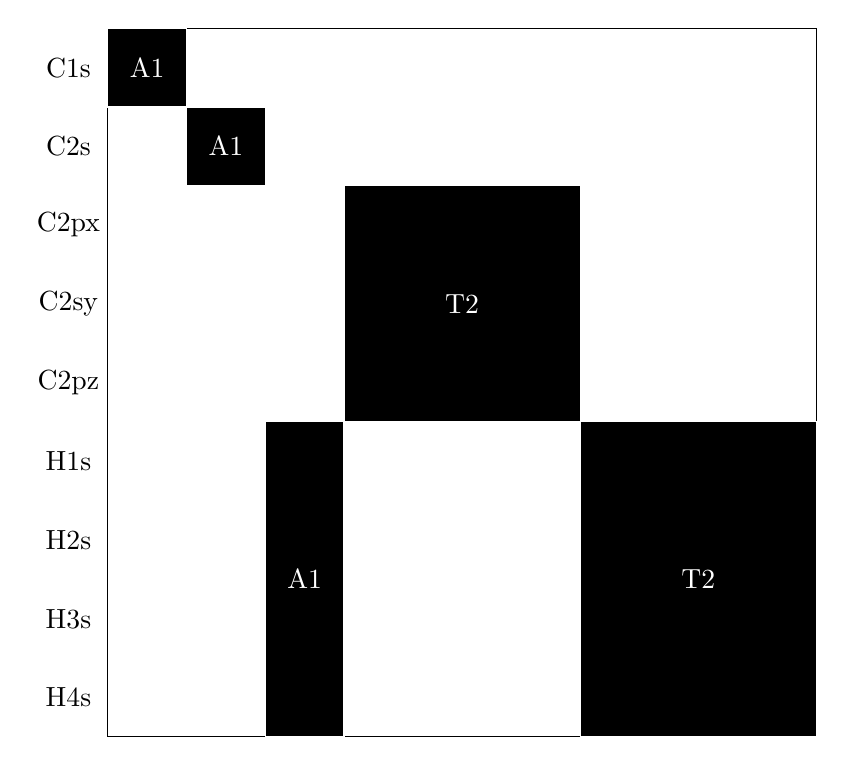
\begin{tikzpicture}
        \node[draw=none,
        rectangle, 
        minimum width = 1cm, 
        minimum height = 1cm
        ](r) at (-5cm,4cm) {C1s};
        \node[draw=none,
        rectangle, 
        minimum width = 1cm, 
        minimum height = 1cm
        ](r) at (-5cm,3cm) {C2s};
        \node[draw=none,
        rectangle, 
        minimum width = 1cm, 
        minimum height = 1cm
        ](r) at (-5cm,2cm) {C2px};
        \node[draw=none,
        rectangle, 
        minimum width = 1cm, 
        minimum height = 1cm
        ](r) at (-5cm,1cm) {C2sy};
        \node[draw=none,
        rectangle, 
        minimum width = 1cm, 
        minimum height = 1cm
        ](r) at (-5cm,0cm) {C2pz};
        \node[draw=none,
        rectangle, 
        minimum width = 1cm, 
        minimum height = 1cm
        ](r) at (-5cm,-1cm) {H1s};
        \node[draw=none,
        rectangle, 
        minimum width = 1cm, 
        minimum height = 1cm
        ](r) at (-5cm,-2cm) {H2s};
        \node[draw=none,
        rectangle, 
        minimum width = 1cm, 
        minimum height = 1cm
        ](r) at (-5cm,-3cm) {H3s};
        \node[draw=none,
        rectangle, 
        minimum width = 1cm, 
        minimum height = 1cm
        ](r) at (-5cm,-4cm) {H4s};
        
        \node[draw,
        rectangle, 
        minimum width = 9cm, 
        minimum height = 9cm
        ](r) at (0cm,0cm) {};

        \node[draw,
        rectangle, 
        color=white,
        fill=black,
        minimum width = 1cm, 
        minimum height = 1cm
        ](r) at (-4cm,4cm) {A1};

        \node[draw,
        rectangle,
        color=white, 
        fill=black,
        minimum width = 1cm, 
        minimum height = 1cm
        ](r) at (-3cm,3cm) {A1};

        \node[draw,
        rectangle,
        color=white,
        fill=black,
        minimum width = 1cm, 
        minimum height = 4cm
        ](r) at (-2cm,-2.5cm) {A1};

        \node[draw,
        rectangle, 
        color=white,
        fill=black,
        minimum width = 3cm, 
        minimum height = 3cm
        ](r) at (0cm,1cm) {T2};

        \node[draw,
        rectangle, 
        color=white,
        fill=black,
        minimum width = 3cm, 
        minimum height = 4cm
        ](r) at (3cm,-2.5cm) {T2};

    \end{tikzpicture}
    \caption{A breakdown of the symmetry orbitals in STO-3G methane into the subspaces 
    present in the T\textsubscript{d} point group.}
\end{figure}

This procedure was implemented and tested on methane with a minimal STO-3G basis set.
It was found that this could accurately assign the MOs and overall wavefunction of
methane the ground state.

To assign a label to each molecular orbital, the character of each orbital in all
subspaces was looked at. This required transforming the molecular orbital coefficients
$\mathbf{C}$ into each subspace $A$ by using the transformation matrix $\mathbf{T}$, 
defined by

\begin{equation}
\tilde{\mathbf{C}}_A = \mathbf{T}^T_A \mathbf{S} \mathbf{C}
\end{equation}
%
, and then summing the coefficients to obtain the character

\begin{equation}
P_A = \sum_{\nu} \left\lvert \tilde{\mathbf{C}}_{A, \mu\nu} \right\lvert  
\end{equation}
%
, where $\mu,\nu$ are indices for the atomic and molecular orbitals respectively. 
The molecular orbital with character equal to 1 in a subspace would then have that
symmetry label, and would be a well defined assignment. However, in practice this was
not always clear cut and so the highest subspace character was taken as the assignment.

The MOs for an optimised methane geometry with an STO-3G basis set was correctly
assigned  - two occupied orbitals and one unoccupied orbital of A1 symmetry,
and three occupied and unoccupied orbitals of T2 symmetry. The overall wavefunction
symmetry can then be expressed as the product of all MO symmetries, reduced with
the reduction formula

\begin{equation}
n = \frac{1}{h} \sum_R \xi_r \left( R \right) \xi_i \left( R \right)
\end{equation}
%
, where $\xi_r, \xi_i$ are the reducible and irreducible representations respectively,
$h$ is the order of the group and $R$ is the subspace. This correctly produced
the overall symmetries of ground state systems for methane, as well as water.

However the assignment of MOs did not work well for excited states, due to the
character from the subspace projection being unclear for many MOs. 
Furthermore, for non-abelian groups, where there are some degenerate E
and T subspaces, this assignment procedure did not work. This is a similar problem 
to the assignment of symmetry for the TD-DFT and EOM-CCSD transitions in the earlier 
benchmarking. Often the reduction of ground state wavefunctions gave non-physical answers.

Extending the symmetry analysis to non-abelian point groups was beyond the scope 
of this work. Altough it would be a useful feature for testing the benchmarking sets,
chlorophyll molecules would be far from symmetric and so this type of assignment 
could not have been expected to have worked. In summary, transitions could not be 
confidently assigned for \dscf with this method.

\subsubsection{\dxtb Benchmarking Results}
\label{subsubsec:imp_of_benchmarking}

After considering this leading error, the assignment of symmetry was based on the
previously used inspection of transition dipole orientations and transition density
plots.

The distributions of absolute errors

\begin{equation}
\epsilon = \Delta E_{\text{method}} - \Delta E_{\text{SCS-CC2}}
\end{equation}
%
for each of the benchmarking methods, as well as a generated distribution of sTDA-xTB
results, are shown in fig-\ref{fig:dxtb_absolute_errors}. The means and standard
deviations are reported in table \ref{table:mean_std_devs}.

\begin{figure}
    \centering
    \includegraphics[scale=0.6]{../../Year_2/test_sets/sTDA_xtb_fit/stda_fit/HCNOF/dxtb_absolute_errors.png}
    \caption{The distributions of errors compared to SCS-CC2 transition energies for the methods
    included in the \dxtb benchmarking.}
    \label{fig:dxtb_absolute_errors}
\end{figure}

\begin{table}
\centering
\begin{tabular}{||c c c||}
    \hline
    Method & Mean / eV & Standard Deviation / eV \\ [0.5ex]
    \hline\hline
    TD-DFT CAM-B3LYP/aug-cc-pVTZ & -0.18 & 0.34 \\
    TD-DFT PBE0/Def2-SVP         & -0.06 & 0.79 \\
    \dscf CAM-B3LYP/aug-cc-pVTZ  & -0.14 & 0.28 \\
    \dscf PBE0/Def2-SVP          & -0.62 & 0.50 \\ 
    TD-GFN1-xTB                  &  0.27 & 1.47 \\ 
    TD-GFN0-xTB                  & -0.41 & 1.32 \\ 
    \dscf GFN1-xTB               & -0.12 & 2.11 \\ 
    \dscf GFN0-xTB               & -1.50 & 1.08 \\
    \code{xtb4stda}              &  4.39 & 1.26 \\  [1ex]
    \hline 
\end{tabular}
\caption{Mean and standard deviations of the errors, in eV, against SCS-CC2
reference data. The \code{xtb4stda} entry represents the eigenvalue difference
method that uses the eigenvalues output from this program.}
\label{table:mean_std_devs}
\end{table}

Overall, both \dxtb methods are inaccurate - far too inaccurate to be used as a 
viable method for transition properties of chlorophyll, or any other system.
The mean error GFN1-\dxtb was -0.12 eV, and has a significant standard deviation
of 2.11 eV. GFN0-\dxtb hd a larger mean error of -1.50 eV, and whilst a slightly
smaller standard deviation of 1.08 eV, this is still well beyond a usable accuracy.

The standard deviation should be well inside the value of the transition energy
(~1.8 eV for \Qy), so a 1 eV accuracy is used as the first test of usuable accuracy.
Next, in order to be accurate enough to predict variations that cannot be attributed
to random noise, the standard deviation must be within the range of excitation energies 
for LHII chlorophylls, which from \ref{fig:chl_energy} can be seen to be around 0.2 eV.
Any more than this and it's uncertain whether the difference between two excitation 
energies for different chlorophyll geometries are due to geometry reasons or due
to random noise.

The DFT methods, both the linear response and the \dscf methods, are still shown
to be accurate at predicting excitation energies, with means and standard deviations
within ranges previously reported in the above sections.

From these results, it's argued that decreasing the level of theory for the electronic
structure dramatically decreases the accuracy of transition properties.
The highest level electronic structure method has the best accuracy. CAM-B3LYP/aug-cc-pVTZ 
TD-DFT and \dscf have mean errors of -0.18 eV and -0.14 eV and standard
deviations of 0.34 and 0.28 eV respectively. Both methods are well within the accuracy
needed to predict geometry-based variations. The outliers in the \dscf results are known 
mixed transitions, as discussed earlier with the ethene dimer system. 
The lower level PBE0/Def2-SVP methods have a marked decrease in accuracy. On going
from higher-level DFT to lower level, the standard deviation approximately doubles 
for both TD-DFT (0.34 eV to 0.79 eV) and \dscf (0.28 eV to 0.50 eV). Again, the
PBE0/Def2-SVP TD-DFT and \dscf are comparable, with standard deviations of 0.79 eV
and 0.59 eV, although the mean for \dscf has a significant shift of -0.62 eV. 
However it's clear that the greater effect on accuracy is due to the change in
response method rather than level of theory of the DFT calculation.
Whilst the same conclusion is not as clear for the semi-empirical methods, the 
large standard deviations of all the GFN based methods fail the first test of
accuracy, and so can be immediately disqualified. They are all too inaccurate to 
justify a more detailed analysis.
Comparing the DFT and GFN based methods, we can see the same trend that lowering
the level of theory gives worse transition properties.

Overall, the most inaccurate method is the eigenvalue difference methods based
orbital energies (eigenvalues of the Hamiltonian diagonalisation) from the \code{xtb4stda}
method. The means and standard deviation was 4.39 eV and 1.26 eV respectively,
a huge difference to the reported values (-0.04 eV and 0.41 eV respectively)\cite{Grimme2016}. 
However it does show that the full sTDA-xTB method can be as accurate as TD-DFT
with a range-based density functional and triple zeta basis sets, and so arguably
the sTDA method, and not the underlying xTB method, makes up a large part of
the accuracy for predicting transition properties. Hence a similar response theory,
based on a different xTB theory, could perform equally well if the xTB theory really
does not factor into obtaining decent accuracy. This is investigated in the next
chapter.

The result that GFN-xTB based methods are not accurate is not unexpected. As opposed
other DFT method, which use \emph{ab initio} or first principle parameters, the
xTB methods were fit to target properties, and so could not be expected to be suitable
for other properties outside the training data \cite{Bannwarth2020}. Whilst GFN-xTB
is better for number and specificity of parameters than many other methods because 
of this "top-down" parameterisation approach, these parameters only extend the
accuracy of predicted properties to different chemical systems (due to a lack 
of pair-wise parameters), and not to different properties altogether.

\section{Conclusions}
The transition properties of a test set of small molecules has been benchmarked 
with multiple \dscf, TD-DFT and high-level methods. It has been shown that DFT 
based \dscf and TD-DFT methods can reproduce the same transition energies and 
transition dipole magnitudes as EOM-CCSD to within reasonable levels
of accuracy. For the set of small molecules, transition energies were predicted
with a mean of less than 0.5 eV, and 0.07 a.u. for transition dipole magnitudes.
Additionally, the issue of breaking the origin independence property of transition
dipoles has been shown to be fixed by using a symmetric orthogonalisation of the 
two originally non-orthogonal states.

For a small set of BChla geometries, it was found that the same level of accuracy
for transition energy could be found between \dscf and TD-DFT, where EOM-CCSD was
too expensive to calculate. The error was well within the range of TD-DFT energy
variation, shown in the high correlation coefficient, and so \dscf could be reasonably
expected to give correct geometry-dependent transition energies. Whilst the accuracy
is slightly reduced for transition dipole moments, the appreciable degree of correlation
implies that qualitative statements would be valid.

With all of the above benchmarking, reliably obtaining and assigning transitions
predicted from \dscf has proved to be an unsolved issue. Either \dscf is formally
unable to predict the correct character of transitions, as showcased in the ethene 
dimer mixed transition outlier, or it is unreliable in finding excited state solutions.
This is best shown in the exclusion of a geometry of chlorophyll that could not
be made to converge to the correct excited state, as well as the necessary use of
Fock damping, altered DIIS procedures and intermediate initial guesses to investigate
whether the convergence could be fixed.

To solve the inability of currently implemented \dscf to assign symmetry labels,
a post-SCF method of assigning MO and full wavefunction symmetry was investigated,
but ultimately proved beyond the scope of this project. Whilst able to assign labels
for small, trivial systems of STO-3G water and methane, non-trivial excited states
and more complex systems did not work. Whilst there is more work that could be done
in this area, it was decided that this should be moved to potential further work
on \dscf methods.

Additionally, whilst DFT based \dscf methods are shown to be accurate, GFN-xTB based methods
were found to be inaccurate, to the point where it cannot be claimed to be a useful
proxy to higher level methods. Due to the similarity in results for linear response and
\dscf methods over a range of electronic structure methods, from high level DFT
to lower level GFN-xTB methods, this drop in accuracy is attributed to the different 
electronic structure theory used, rather than the response methods. This implies
that altering the electronic structure method could lead to great improvements
in the accuracy of a new response method.

The aim of this chapter was to determine whether \dscf methods, which have a simple
gradient theory and are less costly than TD-DFT, could provide a sufficiently accurate
description of transition properties for use in an ab initio exciton framework.
It's been shown that this is true with the condition that the underlying theory
is sufficiently high. The issue of non-orthogonality has shown to have a solution
that does not decrease the speed or accuracy of this method, and whilst the problem
of symmetry assignment is still unsolved, this is not as much of an issue when only
the \Qy transition of chlorophyll, which is well defined by its transition dipole, is 
needed.

However, the fact that higher level DFT is required for accurate transtion properties 
is an issue for simulating a large volume of chlorophyll structures. The efficiency
of these calculations is too low for an exciton framework, which would require in
the region of 1e5 to 1e6 calculations for a full time series of LHII. Semi-emperical
\dscf methods, which would be efficient enough and have tractablegradients, prove
innaccurate in their current form. However, it is demonstrated that a correct electronic
structure and "top-down" parameterisation could make an accurate semi-emperical
method. This is investigated in the following chapter.
